\documentclass{beamer}

\usepackage{HECbeamer}
% \usepackage{pgfpages}
% \pgfpagesuselayout{4 on 1}[letterpaper, landscape, border shrink=5mm]
\usepackage{icomma}
\uselanguage{French}
\languagepath{French}

\title[\color{white}{MATH60604 \S~3 Vraisemblance}]{MATH60604 \\Modélisation statistique \\ \S~3 Vraisemblance}
\author{Léo Belzile}
\date{\today}
\institute{HEC Montréal\\
Département de sciences de la décision}
\date{} 
\newcommand{\AIC}{\ensuremath{\mathsf{AIC}}}
\newcommand{\BIC}{\ensuremath{\mathsf{BIC}}}
\begin{document}
\frame{\titlepage}

\section{Fonction de vraisemblance}
\begin{frame}[fragile]
\frametitle{Vraisemblance}
\bi

\item La \alert{vraisemblance} $L(\bs{\theta})$ est une fonction des paramètres de la loi des observations, $\bs{\theta}$.
\bi \item La vraisemblance est la probabilité d'observer l'échantillon sous le modèle avec $\bs{\theta}$.
\item Les observations sont fixées à leurs valeurs réalisées.
\ei
\item L'estimateur du \alert{maximum de vraisemblance} $\hat{\bs{\theta}}$ est la valeur de $\bs{\theta}$ qui maximise la vraisemblance.
\bi \item soit la valeur pour laquelle l'échantillon observé est le plus probable ou susceptible.
\item raisonnement scientifique: on s'attend à voir ce qu'on observe.
\ei
% \item Quelque soit le modèle que l'on veuille ajuster (incluant des modèles très complexes), il y a toujours des paramètres à \alert{estimer}.
% \item La méthode du \alert{maximum de vraisemblance} permet d'estimer les paramètres de n'importe quel modèle, en maximisant un critère bien précis (la vraisemblance).

\ei
\end{frame}
\begin{frame}[fragile]
\frametitle{Échantillon de loi Bernoulli}
\bi
\item  Supposons que nous voulons estimer la probabilité qu'un événement survienne, sans
aucune variable explicative.    
\item Par exemple, est-ce que le client achète un certain produit ou non, est-ce
qu'un participant à une étude réussit la tâche demandée, etc.

\item On a à disposition un échantillon aléatoire de taille $n$, où $X_i$ suit une loi Bernoulli de paramètre $p \in (0,1)$, 
\begin{align*}
\P{X_i=1}=p , \qquad \P{X_i=0}=1-p.
\end{align*}

\item Par convention, on désigne le résultat « $1$ » par un succès et « $0$ » par un échec.
% \item Il s'agit d'un cas simple où la variable d'intérêt possède seulement deux
% valeurs et où on est intéressé à estimer la probabilité d'avoir le résultat « 1 ».
\ei
\end{frame}

\begin{frame}[fragile]
\frametitle{Probabilité conjointe d'événements binaires}
 Une manière compacte d'écrire la fonction de masse de l'observation $X_i$ est
\begin{align*}
P(X_i=x_i \mid p)=p^{x_i} (1-p)^{(1-x_i)}, \qquad x_i=0, 1.
\end{align*}
 Comme les observations sont indépendantes, la probabilité conjointe d'avoir
un résultat donné est le produit des probabilités pour chaque observation,
\begin{align*}
P(X_1=x_1, \ldots, X_n=x_n\mid p)&=\prod_{i=1}^n \P{X_i=x_i  \mid p}\\&=\prod_{i=1}^n p^{x_i} (1-p)^{(1-x_i)}.
\end{align*}
% \item L'idée de base de la méthode du maximum de vraisemblance est de considérer les valeurs observées
% fixées et de voir cette fonction comme étant une fonction des paramètres (ici, il
% y a un seul paramètre $p$ ).
% \item Cette fonction est la \alert{fonction de vraisemblance} (\textit{likelihood function}).
% \ei
\end{frame}

\begin{frame}[fragile]
\frametitle{Vraisemblance du modèle Bernoulli}
 La fonction de vraisemblance pour un échantillon aléatoire est
\begin{align*}
L(p; \bs{X}) \equiv L(p; \bs{X})&=\prod_{i=1}^n p^{X_i} (1-p)^{(1-X_i)}\\&= p^{\Sigma_{i=1}^n X_i}(1-p)^{n-\Sigma_{i=1}^n X_i}.
\end{align*}
% \item On va habituellement simplifier la notation et seulement utiliser $L( p)$, en
% gardant à l'esprit que c'est une fonction étant donné qu'on considère les
% observations fixes. 
% \item Pour une valeur de $p$ donnée, $L( p)$ est la \alert{probabilité
% d'avoir observé cet échantillon}. 
% \item L'estimation par la méthode du maximum de vraisemblance de $p$ est défini comme étant \alert{la valeur de $p$ qui maximise la fonction de vraisemblance} $L(p)$ . C'est-à-dire, c'est la valeur telle que la probabilité d'avoir observé cet échantillon est la plus grande. 
% \item Autrement dit, l'estimateur de maximum de vraisemblance est la valeur qui rend
% l'échantillon le plus \alert{vraisemblable}, le plus \alert{plausible}.
% \ei
% \end{frame}
% 
% \begin{frame}[fragile]
% \frametitle{Exemple d'introduction à la méthode du maximum de vraisemblance}
% \bi
La vraisemblance est, à une constante de normalisation près, la fonction de masse d'un échantillon de loi binomiale avec $n$ essais et probabilité de succès $p$.
\bi
\item La vraisemblance ne dépend que du nombre de succès observés, peu importe l'ordre des observations. 
\item  L'estimateur du maximum de vraisemblance est la proportion de succès dans l'échantillon.
\ei
Supposons qu'on a $n=10$ observations avec huit succès.
\bi
\item La fonction de vraisemblance est $L(p)=p^8(1-p)^2$.% et l'estimé du maximum de vraisemblance $\hat{p}$ est $0,8$.
\ei
\end{frame}

 \begin{frame}
\frametitle{Graphe de la vraisemblance}
\begin{center}
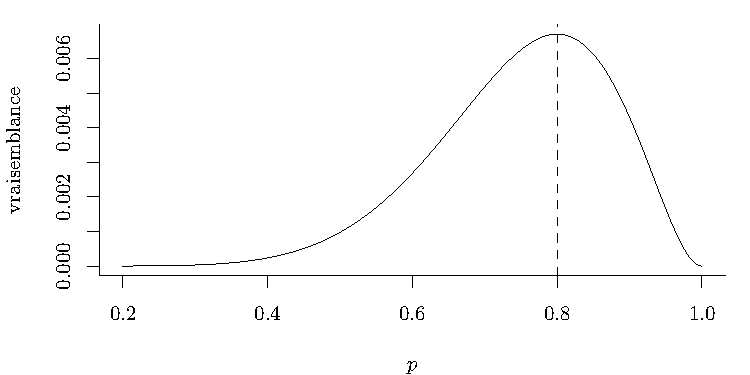
\includegraphics[width = \linewidth]{img/c3/likelihood_fr.pdf}
\end{center}

\end{frame}
% 
% \begin{frame}
% \frametitle{Log-vraisemblance}
% \bi
% \item La maximisation de la vraisemblance est parfois numériquement instable parce qu'on multiplie de petits nombres entre zéro et un.
% \item Comme le logarithme naturel $\log \equiv \ln$ est une fonction
% strictement croissante, maximiser la vraisemblance ou maximiser le log de la
% vraisemblance revient au même.
% \bi 
% \item Le log d'un produit est la somme des logs, soit $\log(ab) =\log(a) +\log(b)$; le produit de $n$ termes devient une somme.
% \item Il est habituellement plus simple de travailler avec une somme plutôt qu'avec
% un produit. 
% \ei 
%  \item On dénote la fonction de \alert{\textbf{log-vraisemblance}} par $\ell(\bs{\theta}) = \log\{L(\bs{\theta})\}$.
% \ei
% 
% \end{frame}

\begin{frame}
\frametitle{Log-vraisemblance d'un échantillon Bernoulli}
\bi
\item Dans notre exemple, la fonction de log-vraisemblance est
\begin{align*}
\ell(p)=\sum_{i=1}^n \log\left\{p^{x_i}(1-p)^{1-xi}\right\}
\end{align*}
\item En utilisant la propriété $\log(a^b)=b\log(a)$, on obtient
\begin{align*}
\ell(p)=\log(p)\sum_{i=1}^n x_i + \log(1-p) \left(n-\sum_{i=1}^n x_i\right).
\end{align*}
\item Dans notre exemple numérique, avec huit succès et deux échecs, la log-vraisemblance est $\ell(p)=8 \log(p) + 2 \log(1-p)$.

\ei
\end{frame}

\begin{frame}
\frametitle{Graphe de la log-vraisemblance $\ell(p)$}
\begin{center}
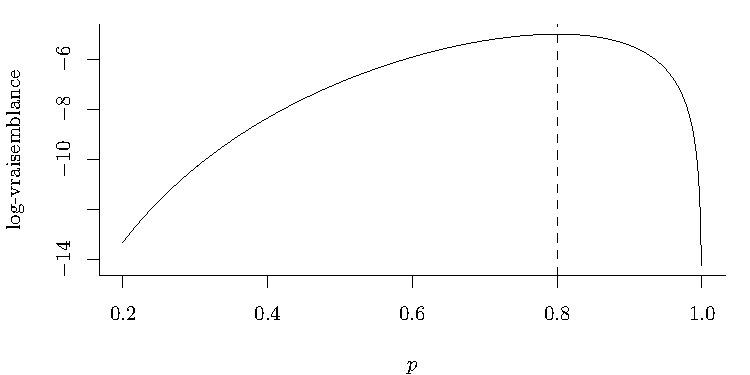
\includegraphics[width = \linewidth]{img/c3/loglikelihood_fr.pdf}
\end{center}
% Même si c'est un peu moins clair que sur le graphe de la vraisemblance, on voit que le maximum est
% aussi atteint au point $p=0.8$ pour cet échantillon.

\end{frame}
% \section{Méthode du maximum de vraisemblance}
% \begin{frame}
% \frametitle{Une remarque sur l'optimisation}
% \bi
% \item En général, le maximum de la fonction de (log-)vraisemblance est obtenu à l'aide d'\alert{algorithmes
% d'optimisation.} 
% \item Heureusement, nous n'avons pas à gérer cela car les algorithmes utilisés dans les logiciels sont habituellement fiables et efficaces pour les modèles vus en classe. 
% \item Pour des modèles plus
% complexes, comme les modèles linéaires généralisés mixtes, la convergence
% des algorithmes d'optimisation peut être plus problématique.
% \ei
% \end{frame}
% 
% \begin{frame}
% \frametitle{Expression analytique pour l'estimateur du maximum de vraisemblance}
% \bi
% \item Dans certains cas simple, il est même possible de dériver une \alert{formule
% analytique} pour l'estimateur maximum de vraisemblance. 
% \item Si la fonction a une dérivée continue en $\bs{\theta}$, l'estimateur du maximum de vraisemblance peut être obtenu
% \bi 
% \item en calculant le gradient (dérivée première) de la (log-)vraisemblance par rapport à $\bs{\theta}$;
% \item trouver le point où le gradient égale zéro;
% \item vérifier que le point est le maximum.
% \ei 
% \ei 
% \end{frame}

\begin{frame}
\frametitle{Estimateur du maximum de vraisemblance pour la probabilité de succès d'une variable Bernoulli}
En dérivant la fonction $\ell( p)$ en fonction de $p$, on obtient
\begin{align*}
\frac{\mathrm{d}}{\mathrm{d}p} \ell(p)=\frac{1}{p} \sum_{i=1}^n x_i-\frac{1}{(1-p)}\left(n-\sum_{i=1}^n x_i \right).
\end{align*}
Si on résoud l'équation $\d \ell(p)/\d p
 =0$, on trouve
\begin{align*}
\widehat{p}=\frac{1}{n} \sum_{i=1}^n x_i = \overline{x}.
\end{align*}
La dérivée seconde,
\begin{align*}
 \frac{\d^2 \ell(p)}{\d p^2} = -\frac{1}{p^2} \sum_{i=1}^n x_i-\frac{1}{(1-p)^2}\left(n-\sum_{i=1}^n x_i \right),
\end{align*}
est négative, donc $L(p)$ atteint un maximum à $\widehat{p}$. L'estimateur du maximum de vraisemblance de $p$ est la \textbf{proportion de succès}.
\end{frame}


\begin{frame}
 \frametitle{Information}
 La courbure de la vraisemblance renseigne sur l'incertitude des estimateurs.
 
 L'information observée est $j(p) = - \d^2 \ell(p)/\d p^2$ et pour notre exemple
 \begin{align*}
j(\widehat{p}) &= \frac{n}{\overline{x}} + \frac{n}{(1-\overline{x})} = \frac{n}{\overline{x}(1-\overline{x})}. 
\end{align*}
La variance de $\widehat{p}$ est $j^{-1}(\widehat{p}) = 0.016$ est l'erreur-type $0.1265$.

L'information de Fisher est
\[
i(\theta) = \frac{n}{p(1-p)}.
\]
\bi \item Pour données indépendantes et identiquement distribuées, l'information cumulative d'un échantillon de taille $n$ est la somme des $n$ contributions individuelles identiques (l'information s'accumule de manière linéaire).
\ei
\end{frame}

\begin{frame}
 \frametitle{Procédures de tests}
 Suppose qu'on veut tester l'hypothèse bilatérale
 \[\Hy_0: p_0 = 0.5 \qquad \text{ versus } \qquad \Hy_a: p_0 \neq 0.5.\]
 
 Trois statistiques basés sur la vraisemblance peuvent être employés pour tester cette hypothèse:
 \bi \item 
la statistique de Wald 
  \[W(p_0) = \frac{(\widehat{p} - p_0)^2}{\Va{\widehat{p}}} = \frac{(\widehat{p}-p_0)^2}{\widehat{p}(1-\widehat{p})/n}\]
  \item  la statistique du score (ou multiplicateurs de Lagrange)
  \[S(p_0) = \frac{U^2(p_0)}{i(p_0)} = \frac{(\widehat{p}-p_0)^2}{p_0(1-p_0)/n}\]
 \item la statistique du rapport de vraisemblance
 \begin{align*}
  R(p_0) &= 2\{\ell(\widehat{p}) - \ell(p_0)\} 
  \\&= 2 \left\{ y\ln \pfrac{\widehat{p}}{p_0} + (n-y)\ln\pfrac{1-\widehat{p}}{1-p_0}\right\}
 \end{align*}
\ei
 \end{frame}
  \begin{frame}
 \frametitle{Illustrations des tests basés sur la vraisemblance}
 \begin{center}
  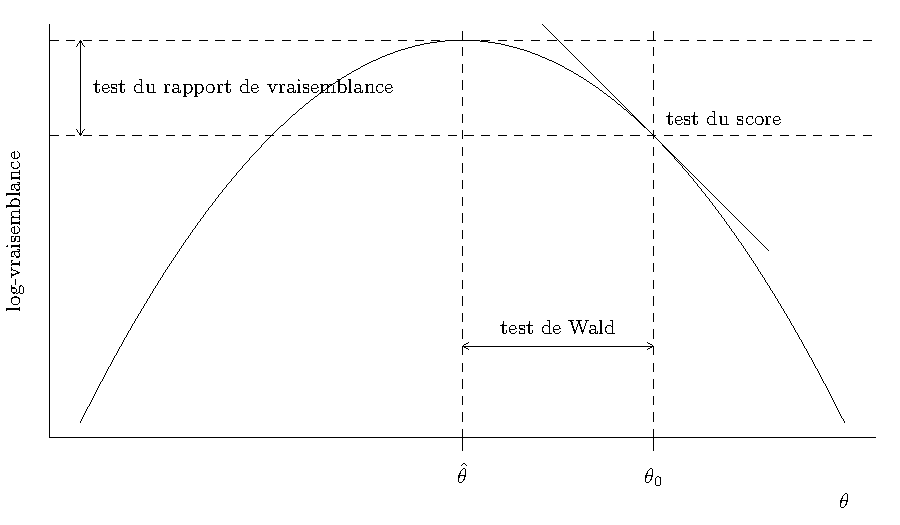
\includegraphics[width = \linewidth]{img/c3/likelihood_tests_fr}
 \end{center}
\end{frame}
 \begin{frame}[fragile]
 \frametitle{Résultats numériques et intervalles de confiance}
 \bi 
 \item Avec 8 succès sur 10 essais, les statistiques valent $W=5.62$, $S=3.6$, $R = 3.855$;
 \item on compare ces valeurs au  $0.95$ quantile de la loi $\chi^2_1$, $3.84$.
 \ei
 \bi \item 
Si la taille de l'échantillon est petite ou que la distribution d'échantillonage de l'estimateur est asymmétrique, le test basé sur la statistique de Wald n'est \alert{pas fiable}.
\item 
 On peut inverser la statistique de Wald pour obtenir un intervalle de confiance à 95\% \[\widehat{p} \pm \mathfrak{z}_{1-\alpha/2}\sqrt{\frac{\widehat{p}(1-\widehat{p})}{n}}\]
 \item Ce dernier vaut $0.8 \pm 1.96 \cdot 0.1265 = [0.55, 1.048]$!
 \item Comparez avec les intervalles de confiance à 95\%
 \bi \item du rapport de vraisemblance, $[0.5005, 0.964]$.
 \item du score, $[0.49, 0.943]$.
  \ei 
  \ei 
  {\footnotesize Résoudre les équations $\{p: S(p) \leq 3.84\}$ et $\{p: R(p) \leq 3.84\}$ numériquement.}
\end{frame}
% 
% \begin{frame}
% \frametitle{Estimation de la moyenne et de la variance d'un échantillon normal}
% Illustration: \textbf{Understanding Maximum Likelihood} par Kristoffer Magnusson, \url{https://rpsychologist.com/d3/likelihood/}
% 
% \bi
% % \item Ainsi, l'estimateur maximum de vraisemblance de $p$ est
% % 
% % \begin{align*}
% % \hat{p}=\frac{1}{n} \sum_{i=1}^n x_i,
% % \end{align*}
% % la \alert{proportion de « 1 » } dans l'échantillon.
% % \item Dans notre exemple numérique, nous avions bien trouvé que $\hat{p}_{mle}=0.8$ car
% % nous avions 80\% de « 1 ».
% % \ei
% % \end{frame}
% % 
% % \begin{frame}
% % \frametitle{Formulation générale de la vraisemblance et propriétés}
% % \bi
% % \item Dans l'exemple de la section précédente, il y avait un seul paramètre ($p$).
% % \item Mais la plupart du temps, le modèle comporte un plus grand nombre de
% % paramètres. 
% % \item Dénotons par $\bs{\theta}$ le $p$-vecteur des paramètres du modèle. 
% % \item L'idée de la méthode est encore la même. En
% % considérant les données fixes, on peut chercher la \alert{valeur de $\bs{\theta}$} qui \alert{maximise
% % la fonction de vraisemblance}, c'est-à-dire, la « probabilité » d'avoir obtenu ces
% % données. 
% % \item Cela revient à chercher la valeur de $\bs{\theta}$ qui maximise la fonction de vraisemblance $L(\bs{\theta})$, ou
% % de manière équivalente, le log de cette fonction $\ell(\bs{\theta})$, la log-vraisemblance.
% % \ei
% % \end{frame}
% % 
% % \begin{frame}
% % \frametitle{Exemple : estimation de la moyenne et de la variance d'une population de loi
% % normale.}
% % \bi
% % \item Voici un deuxième exemple afin de fixer les idées.
% \item Supposons que nous avons un échantillon de taille $n$ tiré d'une loi normale de moyenne $\mu$ et de variance $\sigma^2$, où
% \begin{align*}
% X_i \sim \mathcal{N}(\mu, \sigma^2).
% \end{align*}
% \item Le vecteur de paramètres $\bs{\theta}=(\mu, \sigma^2)$. 
% \item La fonction de densité de la loi normale est
% \begin{align*}
% f(x \mid \bs{\theta})=\frac{1}{(2\pi \sigma^2)^{1/2}}\exp\left\{-\frac{1}{2\sigma^2}(x-\mu)^2\right\}, \qquad x \in \R.                                                                                                                               \end{align*}
% \ei
% \end{frame}
% 
% \begin{frame}
% \frametitle{Exemple : estimation de la moyenne et de la variance d'une population de loi
% normale}
% \bi
% \item Pour un échantillon $\bs{X}=\bs{x}$, la fonction de
% vraisemblance est 
% \begin{align*}
% L(\bs{\theta})=&\prod_{i=1}^n\frac{1}{({2\pi \sigma^2})^{1/2}}\exp\left\{-\frac{1}{2\sigma^2}(x_i-\mu)^2\right\}\\
% =&(2\pi \sigma^2)^{-n/2}\exp\left\{-\frac{1}{2\sigma^2}\sum_{i=1}^n(x_i-\mu)^2\right\}.
% \end{align*}
% \item La log-vraisemblance est
% \begin{align*}
% \ell(\bs{\theta})=-\frac{n}{2}\log(2\pi) -\frac{n}{2}\log(\sigma^2)-\frac{1}{2\sigma^2}\sum_{i=1}^n (x_i-\mu)^2.
% \end{align*}
% % \item Il s'agit d'une fonction de deux variables, $\mu$ et $\sigma^2$. \alert{Les estimateurs maximum de vraisemblance sont
% % obtenus en trouvant les valeurs de $\mu$ et $\sigma^2$ qui maximisent cette fonction.}
% \ei
% \end{frame}
% 
% \begin{frame}
% \frametitle{Expression analytique pour les EMV de l'échantillon normal}
% \bi
% \item Il s'agit d'un autre cas simple où il est possible de résoudre le
% problème analytiquement. En résolvant les \alert{équations du score}
% \begin{align*}
% \frac{\partial}{\partial \mu} \ell(\bs{\theta})=0 , \qquad \frac{\partial}{\partial \sigma^2} \ell(\bs{\theta})=0,
% \end{align*}
% on trouve les estimateurs du maximum de vraisemblance des deux paramètres
% \begin{align*}
% \hat{\mu}=\overline{X}=\frac{1}{n} \sum_{i=1}^n X_i, \qquad \hat{\sigma}^2=\frac{1}{n}\sum_{i=1}^n (X_i-\overline{X})^2.
% \end{align*}
% 
% \ei
% \end{frame}
% 
% \begin{frame}
% \frametitle{Estimer la moyenne et la variance d'une population normale}
% \bi
% \item Intuitivement, on s'attendrait à ce que l'estimateur de la
% moyenne théorique $\mu$ soit la moyenne empirique. 
% \item Par contre, l'estimateur du maximum de vraisemblance de la variance théorique $\sigma^2$ n'est pas la variance empirique 
% \begin{align*}
% S^2=\frac{1}{n-1} \sum_{i=1}^n (X_i-\overline{X})^2.
% \end{align*}
% \item La différence est en fait minime, dans un cas on divise par $n$ et dans l'autre
% par $(n -1)$. 
% \item Les deux estimateurs sont \textbf{convergents}, ce qui veut dire qu'ils convergent vers la même quantité $\sigma^2$ lorsque $n \to \infty$.
% \ei
% \end{frame}
% 
% \begin{frame}
% \frametitle{Biais}
% \bi
% \item Un estimateur de $\theta$ est \textbf{sans biais} si son espérance est $\theta$.
% \bi \item En moyenne, l'estimateur est centré à la vraie valeur, peu importe la taille de l'échantillon $n$.
% \ei 
% \item L'estimateur du maximum de vraisemblance de la moyenne d'un échantillon normal est \alert{sans biais}, c'est-à-dire que
% \begin{align*}
% \E{\hat{\mu}}=\mu.
% \end{align*}
% \item On peut démontrer que $\E{S^2}=\sigma^2$ et donc la variance empirique de l'échantillon est sans biais.
% \item Comme $\hat{\sigma}^2=(n-1)/n S^2$, il en découle que l'estimateur du maximum de vraisemblance de la
% variance est \textbf{biaisé}.
% \ei
% \end{frame}
% 
% %\begin{frame}
% %\frametitle{Propriétés de l'estimateur maximum de vraisemblance}
% %\bi
% %\item Supposons qu'on a un échantillon d'observations de taille $n$ et un modèle qui
% %les relie à un paramètre $\bs{\theta}$ à estimer. Sous certaines conditions, l'estimateur
% %maximum de vraisemblance de $\bs{\theta}$, $\hat{\bs{\theta}}_{mle}$ possède les propriétés suivantes:
% %\bi
% %\vp
% %\item  $\hat{\bs{\theta}}_{mle}$ est convergent, c'est à dire $\hat{\bs{\theta}}_{mle}\rightarrow \bs{\theta}$ lorsque $n \rightarrow \infty$
% %\item $\hat{\bs{\theta}}_{mle}$ est  asymptotiquement de loi normale, c'est-à-dire $\hat{\bs{\theta}}_{mle} \approx \mathcal{N}(\bs{\theta}, \Sigma_{\bs{\theta}})$ où $\Sigma_{\bs{\theta}}$ est la variance (ou matrice de covariance) asymptotique
% %\item $\hat{\bs{\theta}}_{mle}$ possède la plus petite variance asymptotique parmi tous les
% %estimateurs convergents qui sont asymptotiquement de loi normale.
% %\ei
% %\ei
% %\end{frame}
% 
% \begin{frame}
% \frametitle{Régression linéaire ordinaire}
% Si on assume que les aléas sont normaux, l'estimateur des moindres carrés de $\bs{\beta}$ coincide avec l'estimateur du maximum de vraisemblance.
% \bi \item 
% Soit la régression linéaire 
% \begin{align*}
% Y_i=\beta_0+\beta_1 X_{i1}+\beta_2 X_{i2}+\ldots +\beta_p X_{ip} + \eps_i, \qquad  (i=1, \ldots, n),
% \end{align*}
% avec les aléas $ \eps_i\simiid \Cn(0, \sigma^2)$.
% \item Le modèle linéaire a $p+2$ paramètres: $\beta_0, \beta_1, \ldots, \beta_p$ et $\sigma^2$.
% \item La log-vraisemblance est
% \begin{align*}
% \ell(\bs{\theta})&=-\frac{n}{2} \log(2\pi)-\frac{n}{2} \log (\sigma^2)\\& \quad -\frac{1}{2\sigma^2}\sum_{i=1}^n \left(Y_i-\beta_0-\sum_{j=1}^p \beta_jX_{ij}\right)^2.
% \end{align*}
% \ei
% \end{frame}
% 
% 
% \begin{frame}
% \frametitle{Moindres carrés ordinaires et maximum de vraisemblance}
% \bi
% \item Maximiser la log-vraisemblance pour les paramètres $\beta_0, \ldots, \beta_p$ revient à
% minimiser la somme du carré des erreurs,
% \begin{align*}
% \sum_{i=1}^n \left(Y_i-\beta_0-\sum_{j=1}^p \beta_jX_{ij}\right)^2.
% \end{align*}
% \item La fonction objective est la même que celle des moindres carrés.
% \item L'estimateur des moindres carrés $\hat{\bs{\beta}}$ de $\bs{\beta}$ est un estimateur du maximum de vraisemblance.
% \ei
% \end{frame}
% 
% 
% 
% \begin{frame}
% \frametitle{EMV de la variance dans une régression linéaire}
% \bi
% \item L'estimateur du maximum de vraisemblance de la variance $\sigma^2$ est
% \begin{align*}
% \hat{\sigma}^2=\frac{1}{n} \sum_{i=1}^n \left(Y_i-\hat{\beta}_0-\hat{\beta}_1X_{i1}-\cdots-\hat{\beta}_pX_{ip}\right)^2
% \end{align*}
% \item L'estimateur usuel de $\sigma^2$ est plutôt
% \begin{align*}
% S^2=\frac{\mathsf{SS}_e}{n -p-1},
% \end{align*}
% où $p+1$ est le nombre des $\beta$s et $\mathsf{SS}_e$ est la somme du carré des résidus,
% \begin{align*}
% \mathsf{SS}_e = \sum_{i=1}^n e_i^2= \sum_{i=1}^n \left(Y_i-\hat{\beta}_0-\hat{\beta}_1X_{i1}-\cdots-\hat{\beta}_pX_{ip}\right)^2.
% \end{align*} 
% \item $S^2$  est sans biais pour $\sigma^2$, contrairement à $\hat{\sigma}^2$. Les deux estimateurs sont convergents.
% \ei
% \end{frame}
% 
% \begin{frame}
% \frametitle{Régression linéaire ordinaire}
% \bi
% \item L'estimateur du maximum de vraisemblance possède un \alert{léger biais} pour estimer les
% \alert{paramètres de variance}. Ce biais devient négligeable à mesure que 
% la taille d'échantillon augmente si $n \gg p$.
% \item La méthode d'estimation du maximum de vraisemblance restreint (REML, pour
% \textbf{restricted maximum likelihood}) est une variante de la méthode du maximum de vraisemblance qui
% tente de corriger ce biais. Elle est basée sur la vraisemblance d'une combinaison linéaire des observations. 
% \item C'est la méthode que nous allons utiliser pour ajuster les modèles mixtes (Chapitre 7) et on vous recommende son utilisation. C'est également la méthode d'estimation par défaut en \SASlang pour la procédure \code{mixed}.
% \ei
% \end{frame}
% \begin{frame}
% \frametitle{Propriétés de l'estimateur du maximum de vraisemblance}
% Plusieurs propriétés des estimateurs du maximum de vraisemblance (EMV) les rendent attrayants pour l'inférence.
% \be
% \item Les EMV sont \alert{\textbf{convergents}}, c'est-à-dire que l'estimateur converge vers la bonne valeur quand la taille de l'échantillon augmente (\textbf{asymptotiquement sans biais}).
% \item Sous des conditions de régularité, les EMV suivent \alert{\textbf{asymptotiquement}} une loi \alert{\textbf{normale}} lorsque $n$ augmente. 
% \bi \item la loi de l'estimateur est approximativement normale pour $n$ grand;
% \item on peut se servir de cette propriété pour obtenir la loi nulle de test d'hypothèses et dériver des intervalles de confiance.
% \ei
% \item Les EMV sont efficaces: il possèdent la
% \alert{plus petite erreur moyenne quadratique}, ou de manière équivalente la plus petite variance asymptotique qu'il est possible d'atteindre.
% \ee
% \end{frame}
% 
% \begin{frame}
% \frametitle{Matrice de covariance des estimateurs}
% Les dérivées de la vraisemblance encodent de l'information utile sur le modèle.
% \bi 
% \item Le score $S(\bs{\theta}) = \partial \ell(\bs{\theta}) / \partial \bs{\theta}$ est zéro lorsqu'évalué aux estimateurs du maximum de vraisemblance, $S(\hat{\bs{\theta}})=\bs{0}$. 
% \bi \item Cela permet de vérifier qu'on a bien trouvé le maximum de vraisemblance.
% \ei 
% \item 
% La hessienne  $\mathbf{H}(\bs{\theta}) = \partial^2 \ell(\bs{\theta}) / \partial \bs{\theta} \partial \bs{\theta}^\top$ mesure la courbure de la log-vraisemblance.
% % 
% % \item Sous des hypothèses de régularité, la matrice d'information (la variance de la fonction de score) est \[\mathcal{I}(\hat{\bs{\theta}}) = -\E{\mathbf{H}(\bs{\theta})} = \Va{S(\bs{\theta})}.\]
% % \bi 
% % \item On peut estimer la matrice de covariance de  $\hat{\bs{\theta}}$ par $\mathcal{I}^{-1}(\hat{\bs{\theta}})$.
% \item Souvent, on utilise l'information observée, soit moins l'inverse de la hessienne évaluée à l'EMV, $-\mathbf{H}^{-1}(\hat{\bs{\theta}})$, pour l'estimation de la covariance des EMV.
% \bi \item Les \textbf{erreurs-types} de $\hat{\bs{\theta}}$  sont les racines carrées des éléments diagonaux de $-\mathbf{H}^{-1}(\hat{\bs{\theta}})$.
% \ei
% \ei
% \end{frame}
% 
% \section{Tests basés sur la vraisemblance}
% \begin{frame}
% \frametitle{Modèles emboîtés et tests d'hypothèses}
% \bi \item On considère une hypothèse nulle $\Hy_0$ qui impose des contraintes sur les valeurs possibles de $\bs{\theta}$; ces contraintes ne sont pas imposées sous l'alternative $\Hy_1$. 
% \item Pour ce faire, les deux modèles doivent être \textbf{emboîtés}: le modèle sous $\Hy_1$ est le modèle « complet », et le modèle sous $\Hy_0$ le modèle « réduit » qui est un sous-ensemble du modèle complet sur lequel $q$ contraintes sont imposées.
% \item On ajuste les deux modèles et on obtient les estimateurs du maximum de vraisemblance sous $\Hy_1$ et $\Hy_0$, respectivement $\hat{\bs{\theta}}$ et $\hat{\bs{\theta}}_0$.
% \ei 
% 
% 
% \vp\vp
%  {\footnotesize Par exemple, le modèle complet pourrait être un modèle linéaire avec quatre variables explicatives et le modèle réduit avec seulement les deux premiers prédicteurs, ce qui correspond au cas $\Hy_0: \beta_3=\beta_4=0$.
%  
%  }
% %  \end{frame}
% % L'utilisation de la vraisemblance comme critère d'optimisation donne accès à des procédures de tests omnibus.
% % 
% % La fonction de log-vraisemblance $\ell(\bs{\theta})$ est l'ingrédient de base de ces tests.
% % \bi
% % \item on mesure l'écart entre la qualité de l'ajustement sous l'hypothèse nulle (où des contraintes sont imposées sur les valeurs possibles des paramètres) et l'hypothèse alternative.
% % \bi \item Soit $\widehat{\bs{\theta}}_0$ et $\hat{\bs{\theta}}$ les estimateur du maximum de vraisemblance sous $\Hy_0$ et $\Hy_1$, respectivement.
% % \item Par définition, l'EMV maximise la log-vraisemblance et  $\ell(\widehat{\bs{\theta}}_0) \leq \ell(\widehat{\bs{\theta}})$.
% % \item On peut utiliser le \textbf{gradient} de la log-vraisemblance, $S(\bs{\theta}) = \partial \ell(\bs{\theta}) / \partial \bs{\theta}$, soit la \textbf{fonction de score} pour mesurer à quel point l'estimé sous $\Hy_0$ diffère de l'optimum, sachant que  $S(\hat{\bs{\theta}})=\bs{0}$ si le modèle est régulier. 
% % \ei
% % \ei
% % 
% % 
%  \end{frame}
% \begin{frame}
%  \frametitle{Tests dérivés de la vraisemblance}
%  Il y a trois grande classes de tests basés sur la vraisemblance pour comparer des \textbf{modèles emboîtés}
%  \bi \item tests du rapport de vraisemblance, qui mesurent la différence de log-vraisemblance  (\textbf{distance verticale}) entre  $\ell(\hat{\bs{\theta}})$ et $\ell(\hat{\bs{\theta}}_0)$.
%  \item tests de Wald, qui sont basés sur la \textbf{distance horizontale} standardisée entre $\hat{\bs{\theta}}$ et $\hat{\bs{\theta}}_0$.
%  \item le test du score, qui utilise le gradient pondéré de $\ell$, évalué \textbf{uniquement} à $\hat{\bs{\theta}}_0$ (\textbf{dérivée} de $\ell$).
%  \ei
%  Asymptotiquement, tous les tests sont équivalents (au sens où ils mènent aux mêmes conclusions par rapport à $\Hy_0$).
%  
%  Tous ces tests suivent asymptotiquement une loi $\chi^2_q$ si $\Hy_0$ impose $q$ contraintes.
%  \end{frame}
%  \begin{frame}
%  \frametitle{Illustration des tests de vraisemblance}
%  \begin{center}
%   \includegraphics[width = \linewidth]{figures/05-likelihood_tests_fr}
%  \end{center}
% \end{frame}
% 
% 
% % 
% % \begin{frame}
% % \frametitle{Test du rapport de vraisemblance}
% % \bi
% % \item Pour faire un test du rapport de vraisemblance (RV), on considère deux modèles \textbf{emboîtés} : un modèle  « complet » et un modèle « réduit » qui est un cas particulier du modèle complet avec des contraintes (par exemple, certains paramètres nuls). 
% % \item Cette procédure nécessite d'ajuster le modèle sous $\Hy_0$ et $\Hy_1$ pour obtenir les EMV, respectivement $\hat{\bs{\theta}}_0$ et $\hat{\bs{\theta}}$ (avec et sans contraintes).
% % \bi
% % \item La log-vraisemblance maximale du modèle complet (sans contraintes) est $\ell(\hat{\bs{\theta}})$.
% % \item La log-vraisemblance maximale du modèle réduit est $\ell(\hat{\bs{\theta}}_0)$
% % \ei
% % \item {\footnotesize Par exemple, le modèle complet peut être un modèle linéaire avec quatre prédicteurs et le modèle réduit n'inclut que les deux premiers, ce qui revient à fixer $\beta_3=\beta_4=0$.
% % 
% % }
% % \ei
% % \end{frame}
% 
% \begin{frame}
% \frametitle{Test du rapport de vraisemblance}
% La statistique du test du  \textbf{rapport de vraisemblance} est
% \begin{align*}
% D=2\{\ell(\hat{\bs{\theta}}) - \ell(\hat{\bs{\theta}}_0)\}. 
% \end{align*}
% \bi 
% \item Si l'hypothèse nulle $\Hy_0$ est vraie, alors le modèle réduit est une \textbf{simplification adéquate} du modèle complet.
% \item Si $\Hy_0$ est vraie,  $D \stackrel{\cdot}{\sim}\chi^2_q$, où $q$ est le nombre de restrictions imposées.
% \item La procédure de test est extrêmement générale et a des propriétés attractives: invariance aux reparamétrisation (contrairement aux tests de Wald), test uniformément plus puissant, etc.
% \bi 
% \item Le test-$F$ utilisé dans la régression linéaire est équivalent au test du rapport de vraisemblance pour le modèle linéaire.
% \item mais on a utilisé la distribution exacte plutôt que sa contrepartie asymptotique.
% \ei
% \ei
% \end{frame}
% 
% \begin{frame}
%  \frametitle{Tests du score et test de Wald}
%  \textbf{Test du score}
%  \bi \item Bien qure rarement utilisés, les tests du score utilisent le gradient $S(\bs{\theta})$ du modèle complet, évalué à $\hat{\bs{\theta}}_0$. Le test est avantageux si obtenir les EMV $\hat{\bs{\theta}}$ est coûteux ou difficile.
%  \ei
% %  \item Specifically, the statistic takes the form
% %  \begin{align*}
% %   W_s = S(\hat{\bs{\theta}}_0)^\top \mathcal{I}^{-1}(\hat{\bs{\theta}}_0) S(\hat{\bs{\theta}}_0),
% %  \end{align*}
% %  where $S$ and $\mathcal{I}$ are the score and information under the \textbf{alternative hypothesis}.
% \textbf{Tests de Wald}
% \bi 
%  \item La statistique multidimensionnelle de Wald est
%  \begin{align*}
%   W^2 = -(\hat{\bs{\theta}}-\hat{\bs{\theta}}_0)^\top \mathbf{H}^{-1}(\hat{\bs{\theta}})  (\hat{\bs{\theta}}-\hat{\bs{\theta}}_0).
%  \end{align*}
%  \item Quand $\theta$ est unidimensionnel, la statistique de Wald  $W = (\hat{\theta}-\theta_0)/\mathrm{se}(\hat{\theta})$, est souvent rapportée plutôt; cette dernière est approximativement $ \Cn(0,1)$ sous $\Hy_0$.
% \ei
% \end{frame}
% 
% \begin{frame}
%  \frametitle{Intervalles de confiance}
%  
%  \begin{center}
%   \includegraphics[width = \linewidth]{figures/05-likelihood_ci_fr}
%  \end{center}
% 
% \end{frame}
% \begin{frame}
%  \frametitle{Propriétés des intervalles de confiance de la statistique de Wald}
% Les intervalles de Wald bilatéraux à $(1-\alpha)$ pour un seul paramètre $\theta$ sont de la forme \[\hat{\theta} \pm q_{1-\alpha/2}\mathrm{se}(\hat{\bs{\theta}}),\] où $q_{1-\alpha/2}$ est le quantile $1-\alpha/2$ de la loi normale 
% \bi \item Pour un intervalle à $95$\%, on prend le quantile $97,5$\% de la loi normale standard, à savoir $1,96$.
% \ei
%  \bi 
%  \item Les intervalles sont \textbf{symmétriques} par construction.
%  \item Ils peuvent contenir des valeurs impossibles (par ex., des variances négatives).
%  \item Les intervalles changent avec la paramétrisation du modèle: si on veut un intervalle pour une fonction continue $h(\theta)$, alors en général \[\mathsf{CI}_{\mathrm{Wald}}\{h(\theta)\} \neq h\{\mathsf{CI}_{\mathrm{Wald}}(\theta)\}.\]
% \ei
% \end{frame}
% \begin{frame}
% \frametitle{Propriétés des intervalles de confiance basés sur le rapport de vraisemblance}
%  Les intervalles de confiance sont obtenus après une recherche numérique pour les $\theta$ satisfaisant
%   \begin{align*}
%   \theta: 2\{\ell(\hat{\theta}) - \ell(\theta)\} \leq \chi^2_1(1-\alpha),
%  \end{align*}
% où $\chi^2_1(1-\alpha)$ est le quantile $(1-\alpha)$ de la loi $\chi^2_1$.
%  \bi \item Si $\bs{\theta}$ est multidimensionnelle, l'intervalle de confiance pour $\theta_i$ sont dérivés à partir de la vraisemblance profilée (pas couvert).
%  \item Les intervalles sont  \textbf{invariants aux paramétrisations}: \[\mathsf{CI}_{\mathrm{RV}}\{h(\theta)\} = h\{\mathsf{CI}_{\mathrm{RV}}(\theta)\}.\]
%  \item Parce que la vraisemblance est nulle si une valeur de $\theta$ est impossible, lest intervalles n'incluent jamais que des valeurs plausibles de $\theta$.
%  \item En général, les intervalles sont \textbf{asymmétriques} et ont un meilleur taux de couverture.
%  \ei
% 
% \end{frame}
% 
% \begin{frame}
% \frametitle{Comparaisons de modèle avec la vraisemblance}
% \bi 
% \item La vraisemblance peut servir d'ingrédient pour comparer les modèles: 
% \bi 
% \item plus $\ell(\bs{\hat{\theta}})$ est grand, meilleur est l'ajustement. 
% \item donc plus $-2\ell(\bs{\hat{\theta}})$ est petite, meilleur est l'ajustement. 
% \ei
% \bi
% \item Commentaire: plusieurs logiciels rapportent $-2\ell(\bs{\hat{\theta}})$, souvent (incorrectement) dénomée \textbf{déviance}.
% \ei 
% \item La fonction de vraisemblance ne prend pas en compte la complexité du modèle : 
% \bi 
% \item plus le modèle est complexe (avec davantage de paramètres), plus la vraisemblance est élevée. 
% \item ce n'est pas un problème pour la comparaison de modèles emboîtés parce qu'on compare l'ajustement relatif des deux modèles
% \ei 
% \item Il y a un danger de \textbf{surajustement} si on considère seulement la vraisemblance du modèle.
% \ei
% \end{frame}
% \section{Critères d'information}
% \begin{frame}
% \frametitle{Critères d'information}
% 
% Le \AIC{} et le \BIC{} sont deux critères d'information qui mesurent à quel point le modèle est bien ajusté aux données, en  \alert{pénalisant les modèles avec davantage de paramètres}, 
% \begin{align*}
% \AIC{}&=-2\ell(\hat{\bs{\theta}})+2k \\
% \BIC{}&=-2\ell(\hat{\bs{\theta}})+k\log(n),
% \end{align*}
% où $k$ est le nombre de paramètres dans le modèle.
% \bi 
% \item \textbf{Note}: ces critères ne sont pas des tests formels d'hypothèse sur les paramètres.
% \item 
% Plus la valeur de l'\AIC{} (ou du \BIC{}) est  \alert{\textbf{petite}}, \alert{\textbf{meilleur}} est le modèle. 
% 
% \item Ces critères peuvent être utilisés pour comparer des modèles non-emboîtés. Si on veut considérer des modèles avec des distributions sous-jacentes différentes, il faut inclure les constantes de normalisation.
%  \ei
% \end{frame}
% 
% \begin{frame}
% \frametitle{Remarque sur le \AIC{} et le \BIC{}}
% 
% \bi
% \item Le \BIC{} est plus strict que le \AIC{}, puisque la pénalité augmente avec la taille de l'échantillon. Le \BIC{} mène à des modèles plus parcimonieux, avec moins de paramètres.
% \item Le critère \BIC{} est le seul de ces deux critères qui soit \alert{convergent}. Cela veut dire que si l'ensemble des modèles que l'on considère contient le vrai modèle, alors la probabilité que le critère \BIC{} le choisisse tend vers un lorsque $n \to \infty$. 
% \item Tous les modèles sont en général
% une approximation de la réalité. Il est donc peu probable que le vrai modèle
% fasse réellement partie de ceux considérés. 
% \item Certains auteurs trouvent que le
% \BIC{} est quelquefois trop sévère, c'est-à-dire, qu'il choisit des modèles trop
% simples, pour les petites tailles d'échantillons.
% \item De la même manière le \AIC{} sélectionne souvent des modèles (trop) compliqués si la taille de l'échantillon est grande.
%  \ei
% \end{frame}
% % \begin{frame}
% % \frametitle{Outils basés sur la vraisemblance pour comparer des modèles}
% % \bi
% % \item Il arrive très souvent que nous voulons \alert{comparer} différents modèles pour nos données
% % \item Nous
% % avons donc besoin d'outils pour \alert{choisir} le « meilleur » modèle.
% % \item Il existe trois quantités importantes découlant de la méthode du maximum de vraisemblance:
% % \bi
% % \vp
% % \item $-2\ell(\hat{\bs{\theta}}_{mle})$
% % \item AIC
% % \item BIC
% % \ei
% % \ei
% % \end{frame}
% % 
% % \begin{frame}
% % \frametitle{$-2\ell(\hat{\bs{\theta}}_{mle})$}
% % \vp
% % \bi
% % \item Il s'agit de -2 fois la valeur de la log-vraisemblance évaluée au point mle $\hat{\bs{\theta}}_{mle}$, c'est-à-dire, à la valeur du maximum de la fonction. 
% % \item Peut être
% % vue comme étant une \alert{mesure de qualité de l'ajustement du modèle}. Plus elle
% % est petite, mieux c'est. En effet, plus la vraisemblance est grande, mieux c'est.
% % \item Par contre cette mesure ne tient pas compte de la complexité du modèle. On
% % peut en général la rendre aussi petite que l'on veut en utilisant un modèle de
% % plus en plus complexe (avec de plus en plus de paramètres) mais qui souffrira
% % de sur-ajustement (« over-fitting »), et donc qui ne sera pas une bonne
% % représentation de la réalité sous-jacente. 
% % \ei
% % \end{frame}
% % 
% % %\begin{frame}
% % %\frametitle{$-2\ell(\hat{\bs{\theta}}_{mle})$}
% % %\vp
% % %\bi
% % %\item Pour fixer les idées, regardons ce
% % %que vaut $-2\ell(\hat{\bs{\theta}}_{mle})$ dans le cas de la régression linéaire ordinaire. On peut
% % %facilement vérifier que:
% % %\begin{align*}
% % %-2\ell(\hat{\bs{\theta}}_{mle})=n \log(SS_e/n)+n \log(2\pi +1)
% % %\end{align*}
% % %où $SS_e=\sum_{i=1}^n (Y_i-\hat{Y}_i)^2$ est la somme des carrés des erreurs.
% % %\item Ainsi, dans le cas de la régression linéaire
% % %ordinaire, $-2\ell(\hat{\bs{\theta}}_{mle})$ est essentiellement équivalent à mesurer la qualité du
% % %modèle par la somme des carrés des erreurs (le deuxième terme est une
% % %constante). 
% % %\item Mais le problème est que $SS_e$ diminue toujours lorsqu'on ajoute
% % %une variable au modèle (ou au pire reste le même). Il est donc possible de
% % %faire diminuer  $-2\ell(\hat{\bs{\theta}}_{mle})$ en ajoutant de la complexité inutile dans le modèle.
% % % \ei
% % %\end{frame}
% % 
% % \begin{frame}
% % \frametitle{Critères d'information}
% % \vp
% % \bi
% % \item Les critères d'information d'Akaike et bayésien, le AIC et le BIC, 
% % sont des quantités qui mesurent la qualité de l'ajustement du
% % modèle aux données, en \alert{pénalisant pour le nombre de paramètres utilisés}. 
% % \item Le
% % but est de trouver un bon équilibre entre l'ajustement aux données et la
% % parcimonie, et ainsi se prémunir contre le sur-ajustement. Elles sont définies
% % par :
% % \bi
% % \vp
% % \item $AIC=-2\ell(\hat{\bs{\theta}}_{mle})+2 (\text{nombre de paramètres estimés dans le modèle})$
% % \item $BIC=-2\ell(\hat{\bs{\theta}}_{mle})+\log(n) (\text{nombre de paramètres estimés dans le modèle})$
% % \ei
% % \item Leur utilisation est simple. Plus le AIC (ou le BIC) est petit, mieux c'est. 
% % \item Le BIC
% % pénalise plus le nombre de paramètres que le BIC et donc va choisir, soit le
% % même modèle que le AIC, soit un modèle avec moins de paramètres.
% %  \ei
% % \end{frame}
% % 
% % \begin{frame}
% % \frametitle{AIC and BIC}
% % \vp
% % \bi
% % \item Le critère BIC est le seul de ces critères qui est \alert{convergent}. Cela veut dire que
% % si l'ensemble des modèles que l'on considère contient le vrai modèle, alors la probabilité que le critère BIC le choisisse tend vers 1 lorsque $n$ tend vers
% % l'infini. 
% % \item Il faut mettre cela en perspective. Tous les modèles sont en général
% % une approximation de la réalité. Il est donc peu probable que le vrai modèle
% % fasse réellement partie de ceux considérés. 
% % \item Certains auteurs trouvent que le
% % BIC est quelquefois trop sévère, c'est-à-dire, qu'il choisit des modèles trop
% % simples, pour les petites tailles d'échantillons.
% %  \ei
% % \end{frame}
% % 
% % \begin{frame}
% % \frametitle{Test du rapport de vraisemblance (« likelihood ratio test »)}
% % \vp
% % \bi
% % \item On vient de voir que la quantité $-2\ell(\hat{\bs{\theta}}_{mle})$ est une mesure de la qualité de
% % l'ajustement du modèle et qu'on peut s'en servir pour définir des critères de
% % sélection de modèle (AIC et BIC). 
% % \item Mais ces critères ne sont pas des tests
% % d'hypothèses formels au sujet des paramètres. 
% % \item On peut aussi utiliser la
% % quantité $-2\ell(\hat{\bs{\theta}}_{mle})$ pour construire des tests de comparaison de modèles. Afin de simplifier la notation, 
% % on va simplement la noter par $-2\ell$ à partir de maintenant, tout en se rappelant
% % qu'il s'agit de : -2 fois la valeur de la log-vraisemblance évaluée au point mle $\hat{\bs{\theta}}_{mle}$.
% %  \ei
% % \end{frame}
% % 
% % \begin{frame}
% % \frametitle{Test du rapport de vraisemblance (« likelihood ratio test »)}
% % \vp
% % \bi
% % \item Pour effectuer un test LRT, il faut considérer deux modèles emboîtés, c'est-à dire
% % un modèle « complet » et un autre « réduit » qui peut s'obtenir du modèle
% % complet en imposant des contraintes aux paramètres (par exemple que
% % certains d'entre eux sont 0). 
% % \item Il suffit alors de faire la différence des $-2\ell$ des
% % deux modèles. 
% % \item Plus précisément, la procédure consiste à ajuster 2 modèles :
% % \bi
% % \vp
% % \item Le 1er modèle, le modèle « complet ». On note $-2\ell(complet)$ la valeur de $-2\ell$
% % pour ce modèle.
% % \item Le 2ème modèle, le modèle « réduit ». On note $-2\ell(réduit)$ la valeur de $-2\ell$
% % pour ce modèle.
% % \ei
% % \item Par exemple, le  modèle complet est un modèle de régression qui inclut 4 variables et le modele réduit inclut seulement les 2 premières.
% % \ei
% % \end{frame}
% % 
% % \begin{frame}
% % \frametitle{Test du rapport de vraisemblance (« likelihood ratio test »)}
% % \vp
% % \bi
% % \item Le test est basé sur la statistique:
% % \begin{small}
% % \begin{empheq}[box=\mymath]{equation*}
% % D=(-2\ell(reduit))-((-2\ell(complet))
% % \end{empheq}
% % \end{small}
% % 
% % \item L'hypothèse $\Hy_0$ testée par cette statistique est que le modèle réduit et le
% % modèle complet ne sont pas différents.
% % \item Si $\Hy_0$ est vraie, alors la différence des $-2\ell$ suit approximativement la loi du
% % khi-deux avec un nombre de degrés de liberté égal à la différence du nombre
% % de paramètres entre les deux modèles. On peut donc calculer la valeur-$p$ du
% % test en utilisant la distribution du khi-deux.
% % \item Il s'agit donc d'une procédure de test qui est très générale et qui découle de la
% % méthode du maximum de vraisemblance. Nous allons illustrer l'utilisation de
% % ce test dans le prochain chapitre
% % \ei
% % \end{frame}
% % 
% % \begin{frame}
% % \frametitle{Résumé de ce qu'il faut retenir}
% % \bi
% % \item Comprendre ce que la vraisemblance représente
% % \item Comprendre le principe de maximum de vraisemblance
% % \item Outils de comparaison de modèles: AIC/BIC
% % \item Outil de comparaison de modèles: test LRT (Likelihood Ratio Test)
% % \ei
% % \end{frame}

\end{document}
